\documentclass {report}
\usepackage{graphicx}

\begin{document}
\title{Big Graph Tools}
\author{Tian Yong}
\maketitle
\chapter{Introduction}
\section{Introduction}
There are several choices to implement an algorithm to process a large graph:
\begin{itemize}
  \item Crafting a custom distributed infrastructure. This choice leaves machine learning experts repeatedly design a system and implement it.
  \item Relying on an existing distributed computing platform like MapReduce, which is not suit for graph processing.
  \item Using a single-computer graph algorithm library limiting the scale of problems that can addressed.
  \item Using an parallel graph system, fault tolerance or not.
\end{itemize}
\section{Pregel}
The input to a Pregel computation is a directed graph in
which each vertex is uniquely identified by a string vertex
identifier. Each vertex is associated with a modifiable, user
defined value. The directed edges are associated with their
source vertices, and each edge consists of a modifiable, user
defined value and a target vertex identifier.


Pregel computations consist of a sequence of iterations, called \emph{supersteps}. During a superstep the framework invokes a userdefined function for each vertex, conceptually in parallel.
The function specifies behavior at a single vertex $V$ and a
single superstep $S$. It can read messages sent to $V$ in superstep $S-1$, send messages to other vertices that will be received at superstep $S + 1$, and modify the state of $V$ and
its outgoing edges. Messages are typically sent along outgoing edges, but a message may be sent to any vertex whose
identifier is known.  All communication is from superstep $S$ to superstep $S + 1$. In supersteps, vertex can even change the topology of the graph.

Algorithm termination is based on every vertex voting to
halt. In superstep 0, every vertex is in the active state; all
active vertices participate in the computation of any given
superstep. A vertex deactivates itself by voting to halt. This
means that the vertex has no further work to do unless triggered externally, and the Pregel framework will not execute
that vertex in subsequent supersteps unless it receives a message. If reactivated by a message, a vertex must explicitly deactivate itself again. The algorithm as a whole terminates
when all vertices are simultaneously inactive and there are
no messages in transit. This state transition model is illustrated in figure \ref{SMachine}.


\begin{figure}
  \centering
  % Requires \usepackage{graphicx}
  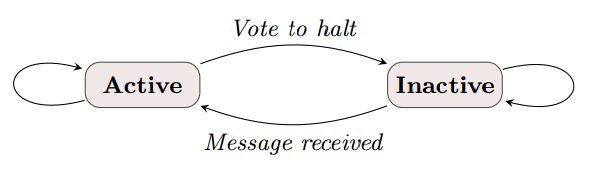
\includegraphics[width=\textwidth]{pregel_vertext_machine.PNG}\\
  \caption{Pregel Vertext State Machine}\label{SMachine}
\end{figure}

Figure \ref{pregel_max} illustrates these concepts using a simple example:
given a strongly connected graph where each vertex contains
a value, it propagates the largest value to every vertex. In
each superstep, any vertex that has learned a larger value
from its messages sends it to all its neighbors. When no
further vertices change in a superstep, the algorithm terminates
\begin{figure}
  \centering
  % Requires \usepackage{graphicx}
  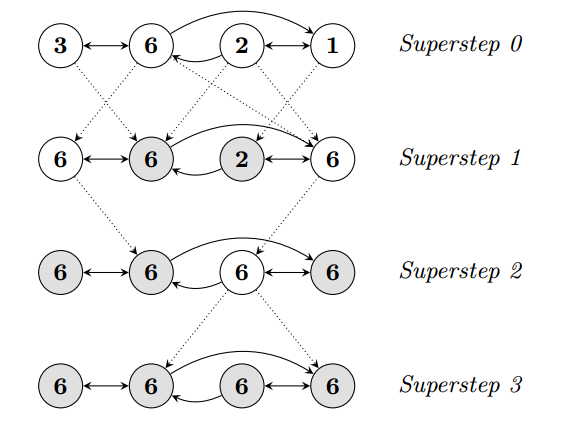
\includegraphics[width=\textwidth]{pregel_max_example.PNG}\\
  \caption{Maximum Value Example. Dotted lines
are messages. Shaded vertices have voted to halt.}\label{pregel_max}
\end{figure}


\subsection{Topology Mutations}
Some graph algorithms need to change the graph's topology. A clustering algorithm, for example, might replace each
cluster with a single vertex, and a minimum spanning tree
algorithm might remove all but the tree edges. User defined function can not only send messages, but also can 
issue requests to add or remove vertices or edges.


Multiple vertices may issue conflicting requests in the same
superstep. To solve this problem, Pregel use two mechanisms to achieve
determinism: 
\begin{itemize}
  \item Partial ordering. As with messages, mutations become elective in the superstep after the requests were
  issued. Within that superstep removals are performed first, with edge removal before vertex removal. Then additions follow, with vertex addition before edge addition. This partial ordering yields deterministic results for most conflicts.
  \item Handlers. The remaining conflicts are resolved by user-defined handlers. For these conflicts, system have a default random resolution. Butt users with special needs may specify a better conflict resolution policy by defining an appropriate handler method.
\end{itemize}

\section{GraphLab}
\section{PowerGraph}
\section{Graphchi}
\end{document}
